% ----------------------------------------------------------
\section{Correção das leituras do sensor CO-B4 com as medições de referência}
% ----------------------------------------------------------

A partir dos dados de referência e das leituras de concentração e temperatura adquiridas pelo monitor em questão, foi realizada uma busca em \textit{grid} para encontrar as melhores combinações de parâmetros e variáveis de entrada aos modelos de regressão. As variáveis que foram testadas como entrada foram as leituras de concentração do sensor CO-B4 e a temperatura no interior da câmara de medição. Na Tabela \ref{tab:data-co-br-calib-results} resumem-se os melhores modelos encontrados pela busca em \textit{grid} para corrigir as leituras do sensor CO-B4. Os mesmos resultados são ilustrados graficamente na Figura \ref{fig:data-co-b4-models-performance} que apresenta o desempenho dos modelos e as variáveis de entrada considerando os valores de r2, RMSE e MAE.

\begin{table}[h!]
    \caption{Resultados da calibração do sensor CO-B4}
    \centering
    \begin{tabularx}{0.95\textwidth}[h!]{
         >{\raggedright\hsize=.2\hsize\arraybackslash}X
         >{\raggedright\hsize=.7\hsize\arraybackslash}X 
         >{\raggedright\hsize=.4\hsize\arraybackslash}X
         >{\raggedright\hsize=.4\hsize\arraybackslash}X 
         >{\raggedright\hsize=.3\hsize\arraybackslash}X 
         >{\raggedright\hsize=.3\hsize\arraybackslash}X }
        \hline
        Var. & Modelo & R2 & RMSE & MAE & $\rho$\\ [0.5ex]
        \hline
        CO & \textbf{MLP}: & -0.45 ± 0.25 & -0.06 ± 0.01 & -0.05 & 0.47 \\ [0.5ex]
           & \textbf{MLR} & -0.63 ± 0.48 & -0.07 ± 0.01 & -0.05 & 0.33 \\ [0.5ex]
           & \textbf{KNN:} & -0.48 ± 0.29 & -0.06 ± 0.01 & -0.05 & 0.46 \\ [0.5ex]
           & \textbf{RF:} & -0.61 ± 0.35 & -0.07 ± 0.01 & -0.05 & 0.39 \\ [0.5ex]
        \hline
        CO, T & \textbf{MLP:} & -0.65 ± 0.40 & -0.07 ± 0.01 & -0.05 ± 0.01 & 0.50 \\ [0.5ex]
              & \textbf{MLR:} & -0.68 ± 0.47 & -0.07 ± 0.01 & -0.05 & 0.31 \\ [0.5ex]
              & \textbf{KNN:} & -0.63 ± 0.38 & -0.07 ± 0.01 & -0.05 & 0.53 \\ [0.5ex]
              & \textbf{RF:} & -0.63 ± 0.43 & -0.07 ± 0.01 & -0.05 & 0.47 \\ [0.5ex]
        \hline
    \end{tabularx}
    \label{tab:data-co-br-calib-results}
\end{table}

\begin{figure}[h]
    \centering
    \caption{Resultados dos modelos de regressão aplicados as leituras do sensor CO-B4}
    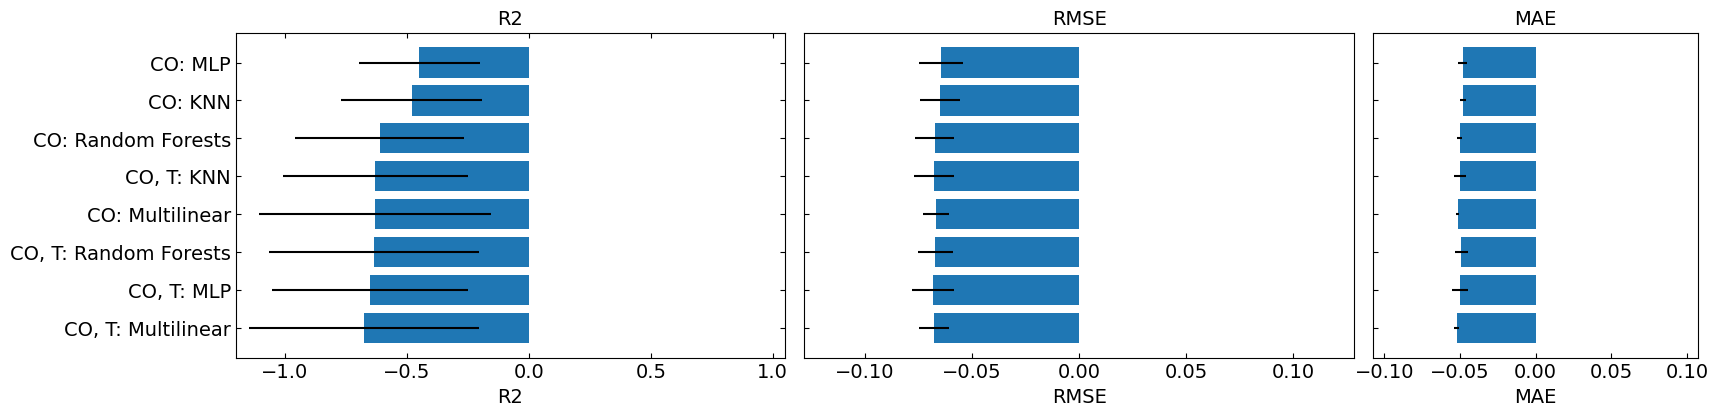
\includegraphics[width=\textwidth]{chapters/4-CALIBRAÇÃO MÚLTIPLOS SENSORES/Figuras/co-b4-models-performance.png}
    \label{fig:data-co-b4-models-performance}
\end{figure}

Como se observa, todas as variantes de modelos e variáveis de entrada apresentaram valores de R2 negativos, indicando que nenhum dos modelos foi capaz de explicar a variância na variável dependente, i.e. a concentração real. Contudo, os modelos não lineares produziram maiores coeficientes de correlação do que as regressões lineares, e de igual modo, os modelos não lineares que incluíram a temperatura, apresentaram melhorias na correlação em comparação com os que não consideraram a temperatura como variável de entrada. Os maiores coeficientes de Spearman foram de 0.53 com uma regressão KNN considerando a temperatura, e de 0.50 utilizando uma rede neural MLP também considerando a temperatura. As Figuras \ref{fig:data-co-T-reference-corr-KNN} e \ref{fig:data-co-T-reference-corr-MLP} apresentam os resultados ao aplicar os modelos de k Vizinhos mais Próximos e Perceptron Multicamadas.

\begin{figure}[h]
    \centering
    \caption{Gráfico de dispersão das leituras do sensor CO-B4 e a estação de referência após aplicar modelos de regressão considerando a temperatura}
    \begin{subfigure}{0.495\textwidth}
        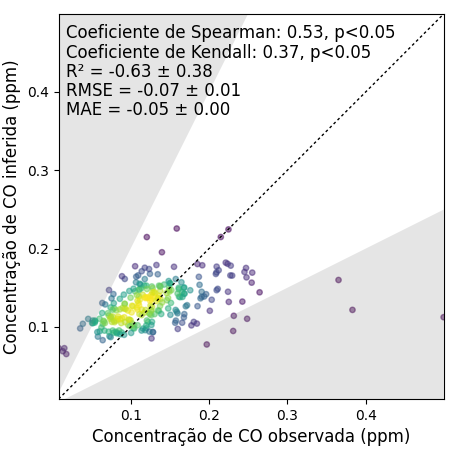
\includegraphics[width=\textwidth]{chapters/4-CALIBRAÇÃO MÚLTIPLOS SENSORES/Figuras/co-b4-T-KNN-Regression.png}
        \caption{Utilizando regressão pelos k Vizinhos mais Próximos}
        \label{fig:data-co-T-reference-corr-KNN}
    \end{subfigure}
    \hfill
    \begin{subfigure}{0.495\textwidth}
        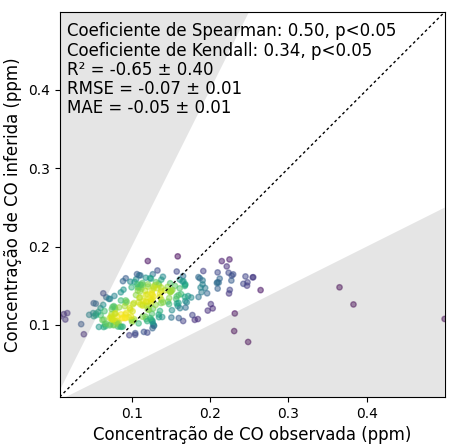
\includegraphics[width=\textwidth]{chapters/4-CALIBRAÇÃO MÚLTIPLOS SENSORES/Figuras/co-b4-T-MLP-Regression.png}
        \caption{Utilizando uma rede neural Perceptron Multicamadas}
        \label{fig:data-co-T-reference-corr-MLP}
    \end{subfigure}
\end{figure}

\begin{figure}[h!]
    \centering
    \caption{Desempenho dos modelos de regressão aplicados para inferir as leituras de concentração de \acrshort{co} medidas pela estação de referência}
    \begin{subfigure}{\textwidth}
        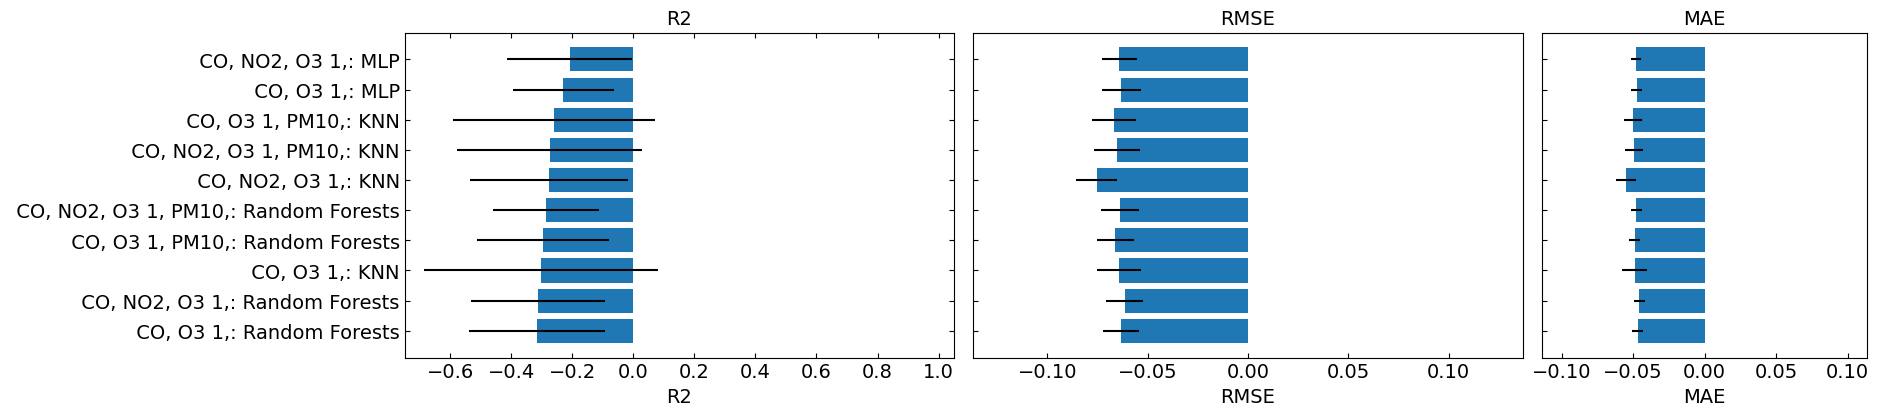
\includegraphics[width=\textwidth]{chapters/4-CALIBRAÇÃO MÚLTIPLOS SENSORES/Figuras/co-all-models-performance.png}
        \caption{Valores de R2, RMSE e MAE obtidos pelos 10 modelos com maiores valores de R2}
        \label{fig:data-co-all-models-performance}
    \end{subfigure}
    \begin{subfigure}{\textwidth}
        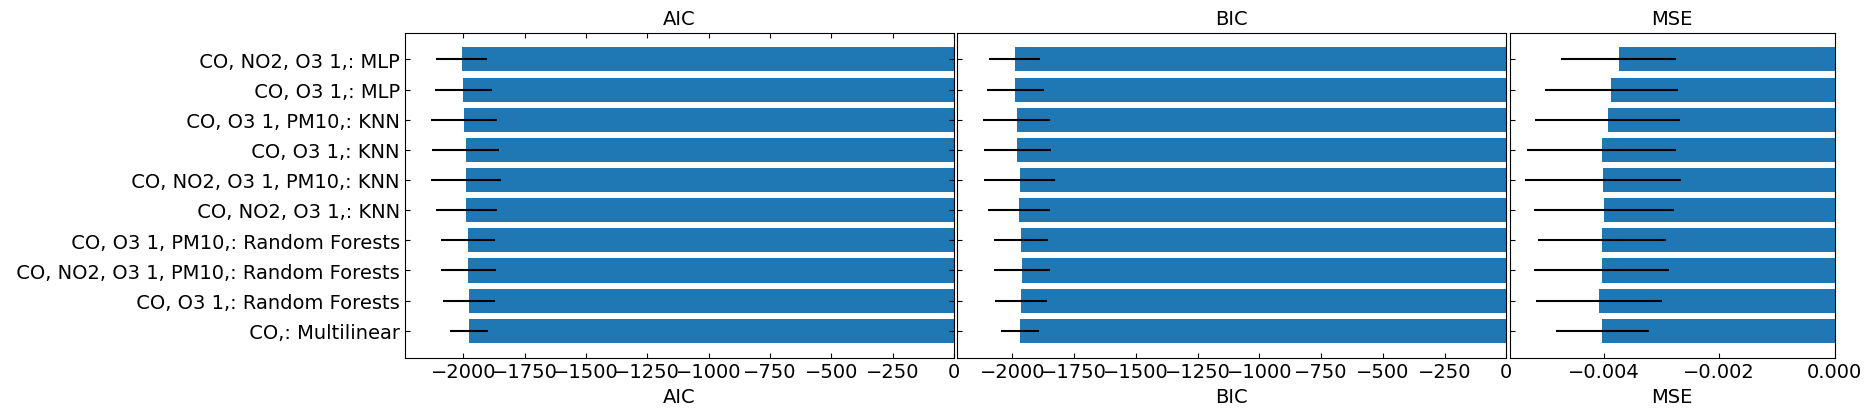
\includegraphics[width=\textwidth]{chapters/4-CALIBRAÇÃO MÚLTIPLOS SENSORES/Figuras/co-all-models-complexity.png}
        \caption{Modelos com menores valores de \acrshort{aic} e \acrshort{bic}}
        \label{fig:data-co-all-models-complexity}
    \end{subfigure}
    \label{fig:data-co-all-models-performance-comlexity}
\end{figure}

% ----------------------------------------------------------
\section{Cálculo da concentração de Monóxido de Carbono a partir das leituras do arranjo de sensores de gases}
% ----------------------------------------------------------

A Figura \ref{fig:data-co-all-models-performance} apresenta os valores de R2 dos 10 melhores modelos de calibração calculados para as leituras de \acrshort{co}. Observa-se que apesar do valor médio de R2 obtido nas validações cruzadas continuar sendo negativo, obtiveram-se máximos de até aproximadamente 0.1 para alguns conjuntos de dados de teste nas validações cruzadas. Em geral os modelos que produziram os melhores resultados foram baseados em regressões pelos k vizinhos mais próximos e redes neurais Perceptron Multicamadas. Com relação as variáveis de entrada dos modelos, todos os que produziram melhores resultados consideraram as leituras do sensor 1 de \acrshort{o3}. Nenhum deles considerou a temperatura.

\begin{figure}[h!]
    \centering
    \caption{Gráfico de dispersão das leituras do múltiplos sensores e a estação de referência para medição de \acrshort{co}}
    \begin{subfigure}{0.495\textwidth}
        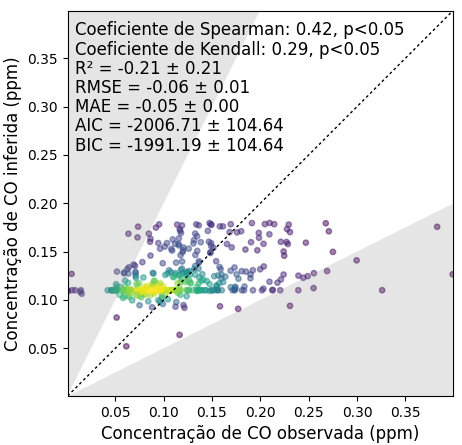
\includegraphics[width=\textwidth]{chapters/4-CALIBRAÇÃO MÚLTIPLOS SENSORES/Figuras/CO-co-no2-o31-mlp-Regression.png}
        \caption{Utilizando modelo de regressão com uma rede neural Perceptron Multicamadas; variáveis independentes: leituras de sensores CO-B4, NO2-B43F e OX-B431 (1)}
        \label{fig:data-co-no2-o31-reference-corr-MLP}
    \end{subfigure}
    \hfill
    \begin{subfigure}{0.495\textwidth}
        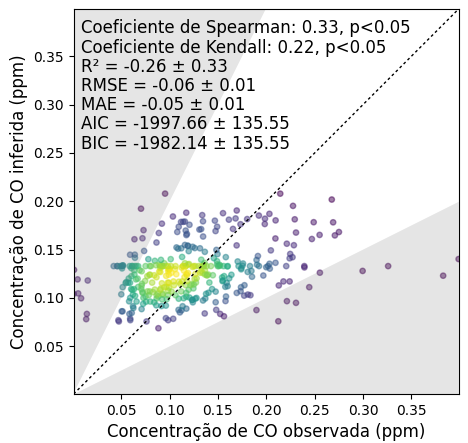
\includegraphics[width=\textwidth]{chapters/4-CALIBRAÇÃO MÚLTIPLOS SENSORES/Figuras/CO-co-o31-pm10-knn-Regression.png}
        \caption{Utilizando modelo de regressão pelos k vizinhos mais próximos; variáveis independentes: leituras de sensores CO-B4, OX-B431 (1) e de \acrshort{mp10} medido pelo OPC-N3}
        \label{fig:data-co-o31-mp10-reference-corr-KNN}
    \end{subfigure}
\end{figure}

Ao comparar os modelos em termos de sua complexidade, observa-se uma sobreposição entre os que desempenharam melhor em termos de representação dos dados originais (maiores valores de R2) e os que desempenharam melhor em termos de complexidade (menores valores de AIC e BIC). A Figura \ref{fig:data-co-all-models-complexity} compara os valores de \acrshort{aic}, \acrshort{bic} e \acrshort{mse} dos 10 modelos que obtiveram menores valores de AIC. Por último as Figuras \ref{fig:data-co-no2-o31-reference-corr-MLP} e \ref{fig:data-co-o31-mp10-reference-corr-KNN} mostram gráficos de dispersão entre os valores de saída dos modelos de calibração e os dados de referência de \acrshort{co}. Os gráficos mostram os resultados dos modelos com melhores valores de R2.